% ================================================================
% The Retrieve and Connect version of latex/starters/targeted/KS4/percentages/percentagesWithMultipliersStarters.tex
%
% This is the same deck as the one above, made by renaming the titles in it.
% Every slide that was a numbered starter is now titled
% "Retrieve and Connect", and the word is renamed wherever else a title
% used it. Nothing outside a title has been changed.
%
%   made from           latex/starters/targeted/KS4/percentages/percentagesWithMultipliersStarters.tex
%   retitling rules     version 1
%
% Please don't edit this file. It is written again from the one it was
% made from whenever that changes, so an edit here would be lost - edit
% that file instead and this one follows.
% ================================================================
\documentclass{beamer}
\usepackage{tikz}
\usetikzlibrary{calc}
\usetikzlibrary{decorations.pathreplacing}
\usepackage{pgfplots}
\pgfplotsset{compat=1.18}
\usepackage{xcolor}
\usepackage{multicol}
\usepackage{amsmath}

\setbeamertemplate{navigation symbols}{}
\setbeamersize{text margin left=0.4cm, text margin right=0.4cm}
\setlength{\multicolsep}{4pt}
\setlength{\columnsep}{14pt}
\renewcommand{\arraystretch}{0.92}

% ================================================================
% Answer-overlay helpers
% ================================================================
\newcommand{\ablank}[1]{%
  \alt<2>{\textcolor{red}{#1}}{\underline{\phantom{#1}}}%
}
\newcommand{\ashow}[1]{\uncover<2->{\textcolor{red}{\small #1}}}
\newcommand{\ashowq}[1]{\alt<2->{\textcolor{red}{\small #1}}{?}}

% Answers drawn straight on to a TikZ diagram, revealed on overlay 2 like \ashow.
% Space is reserved on overlay 1, so the diagram does not move between slides.
\usetikzlibrary{overlay-beamer-styles}
\tikzset{
  ans/.style     = {red, thick, visible on=<2->},
  ansfill/.style = {red!15, visible on=<2->},
  anslab/.style  = {red, font=\tiny, visible on=<2->},
}

% Every question list on these slides is tight, so that the diagram column and
% the question column both finish inside the slide.
\newcommand{\tightlist}{%
  \setlength{\itemsep}{0pt}\setlength{\parskip}{0pt}\setlength{\topsep}{0pt}%
}

% Braces over and under the bar models. The whole percentage goes above the bar
% and the percentage after the change goes below it.
\tikzset{
  topbrace/.style    = {decorate, decoration={brace, amplitude=4pt}, thick},
  bottombrace/.style = {decorate, decoration={brace, amplitude=4pt}, thick},
}

% The boxes and arrows the flow charts are built from.
\tikzset{
  fbox/.style  = {draw, rounded corners=2pt, minimum width=1.55cm,
                  minimum height=0.42cm, inner sep=1pt, font=\small},
  farrow/.style = {->, thick},
  flab/.style   = {font=\scriptsize, inner sep=1.5pt},
  rbox/.style   = {draw, rounded corners=2pt, minimum width=1.2cm,
                   minimum height=0.42cm, inner sep=1pt, font=\small},
  fwdarc/.style = {->, thick, bend left=32},
  bckarc/.style = {->, thick, red!70!black, bend left=32},
}

\title{Percentages with Multipliers: Retrieve and Connects}
\author{}
\date{}

\begin{document}

\frame{\titlepage}

%------------------------------------------------------------------
% STARTER 1: Multipliers for an increase and a decrease
%------------------------------------------------------------------
\begin{frame}[t]{Retrieve and Connect}
\begin{columns}[T]

\column{0.36\textwidth}
\begin{center}
\vspace{-0.9em}
{\footnotesize\textbf{Write the multiplier\\ under each bar model.}}\\[0.4em]
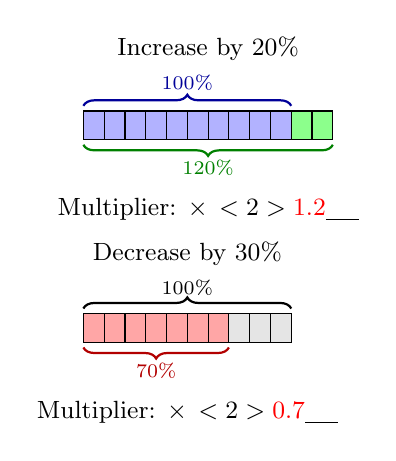
\begin{tikzpicture}[scale=0.66, every node/.style={font=\scriptsize}]

% ---- Increase of 20%: a bar of 12 tenths ----
\node[font=\small] at (2.4,1.75) {Increase by $20\%$};
\draw[topbrace, blue!60!black] (0,0.65) -- (4.0,0.65);
\node[blue!60!black] at (2.0,1.10) {$100\%$};
\foreach \i in {0,...,11}{
  \ifnum\i<10
    \fill[blue!30] (\i*0.4,0) rectangle ++(0.4,0.55);
  \else
    \fill[green!45] (\i*0.4,0) rectangle ++(0.4,0.55);
  \fi
  \draw (\i*0.4,0) rectangle ++(0.4,0.55);
}
\draw[bottombrace, green!50!black] (4.8,-0.10) -- (0,-0.10);
\node[green!50!black] at (2.4,-0.55) {$120\%$};
\node[font=\small] at (2.4,-1.35) {Multiplier: $\times\,\ablank{1.2}$};

% ---- Decrease of 30%: a bar of 10 tenths, 3 taken away ----
\node[font=\small] at (2.0,-2.20) {Decrease by $30\%$};
\draw[topbrace] (0,-3.25) -- (4.0,-3.25);
\node at (2.0,-2.85) {$100\%$};
\foreach \i in {0,...,9}{
  \ifnum\i<7
    \fill[red!35] (\i*0.4,-3.90) rectangle ++(0.4,0.55);
  \else
    \fill[gray!20] (\i*0.4,-3.90) rectangle ++(0.4,0.55);
  \fi
  \draw (\i*0.4,-3.90) rectangle ++(0.4,0.55);
}
\draw[bottombrace, red!70!black] (2.8,-4.00) -- (0,-4.00);
\node[red!70!black] at (1.4,-4.45) {$70\%$};
\node[font=\small] at (2.0,-5.25) {Multiplier: $\times\,\ablank{0.7}$};

\end{tikzpicture}
\end{center}

\column{0.64\textwidth}
\vspace{-1.8em}
\footnotesize
\begin{enumerate}\tightlist
\begin{multicols}{2}
  \item Write $0.35$ as a percentage and as a fraction in its simplest form.
        \ashow{$35\% = \tfrac{7}{20}$}
  \columnbreak
  \item Write $\dfrac{3}{8}$ as a decimal and as a percentage.
        \ashow{$0.375 = 37.5\%$}
\end{multicols}
  \item Complete the table of multipliers.
  \vspace{0.3em}
  \begin{center}
  {\renewcommand{\arraystretch}{1.25}\setlength{\tabcolsep}{6pt}
  \begin{tabular}{c|c|c}
    Change & New amount & Multiplier\\ \hline
    increase of $20\%$ & $120\%$ & $1.2$\\
    increase of $5\%$  & \ablank{$105\%$} & \ablank{$1.05$}\\
    decrease of $30\%$ & $70\%$  & \ablank{$0.7$}\\
    decrease of $8\%$  & \ablank{$92\%$} & \ablank{$0.92$}
  \end{tabular}}
  \end{center}
  \vspace{0.4em}
\begin{multicols}{2}
  \item Increase \pounds240 by $15\%$.
        \ashow{$240\times1.15=$ \pounds276}
  \columnbreak
  \item Reduce \pounds45 by $30\%$.
        \ashow{$45\times0.7=$ \pounds31.50}
\end{multicols}
  \item A school has 850 pupils. The roll rises by $6\%$. How many pupils now?
        \ashow{$850\times1.06=901$ pupils}
  \item Toby says ``an increase of $10\%$ is $\times1.1$, so a decrease of $10\%$ is $\times0.1$''.
        Explain why he is wrong and give the correct multiplier.
        \ashow{$\times0.1$ leaves only $10\%$, a decrease of $90\%$. A decrease of $10\%$ leaves $90\%$, so $\times0.9$.}
\end{enumerate}
\end{columns}
\end{frame}

%------------------------------------------------------------------
% STARTER 2: Chains of multipliers and percentage change
%------------------------------------------------------------------
\begin{frame}[t]{Retrieve and Connect}
\begin{columns}[T]

\column{0.33\textwidth}
\begin{center}
\vspace{-0.4em}
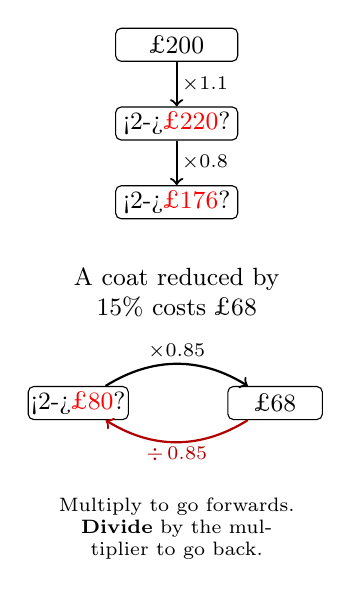
\begin{tikzpicture}[scale=1, every node/.style={font=\scriptsize}]

% ---- Chain of two multipliers ----
\node[fbox] (a0) at (0,0) {\pounds200};
\node[fbox] (a1) at (0,-1.0) {\ashowq{\pounds220}};
\node[fbox] (a2) at (0,-2.0) {\ashowq{\pounds176}};
\draw[farrow] (a0) -- node[flab,right] {$\times 1.1$} (a1);
\draw[farrow] (a1) -- node[flab,right] {$\times 0.8$} (a2);

% ---- Reversing a multiplier ----
\node[font=\small, text width=3.5cm, align=center] at (0,-3.15)
  {A coat reduced by $15\%$ costs \pounds68};
\node[rbox] (b0) at (-1.25,-4.55) {\ashowq{\pounds80}};
\node[rbox] (b1) at ( 1.25,-4.55) {\pounds68};
\draw[fwdarc] (b0) to node[flab, above] {$\times 0.85$} (b1);
\draw[bckarc] (b1) to node[flab, below] {$\div\, 0.85$} (b0);
\node[font=\scriptsize, text width=3.5cm, align=center] at (0,-6.15)
  {Multiply to go \mbox{forwards}. \textbf{Divide} by the multiplier to go back.};

\end{tikzpicture}
\end{center}

\column{0.67\textwidth}
\vspace{-1.8em}
\footnotesize
\begin{enumerate}\tightlist
\begin{multicols}{2}
  \item Write $45\%$ as a decimal and $0.06$ as a percentage.
        \ashow{$0.45$ and $6\%$}
  \columnbreak
  \item Write $\dfrac{7}{20}$ as a percentage.
        \ashow{$35\%$}
\end{multicols}
\begin{multicols}{2}
  \item Write the missing prices in the boxes of the first flow chart.
        \ashow{\pounds220 then \pounds176}
  \columnbreak
  \item Write the multiplier for an increase of $3.5\%$.
        \ashow{$\times1.035$}
\end{multicols}
  \item A bike costs \pounds180. The price rises by $10\%$, then the new price falls by $10\%$.
        Find the final price, and the single multiplier for the two changes together.
        \ashow{$180\times1.1\times0.9=$ \pounds178.20; $1.1\times0.9=0.99$, a $1\%$ decrease}
\begin{multicols}{2}
  \item Write the coat's original price in the empty box of the second flow chart.
        \ashow{$68\div0.85=$ \pounds80}
  \columnbreak
  \item A meal costs \pounds42 after a $20\%$ service charge. Find the price before the charge.
        \ashow{$42\div1.2=$ \pounds35}
\end{multicols}
  \item A jacket has $20\%$ off, then a further $10\%$ off at the till, and costs \pounds180.
        Find the original price.
        \ashow{$0.8\times0.9=0.72$, so $180\div0.72=$ \pounds250.}
\end{enumerate}
\end{columns}
\end{frame}

%------------------------------------------------------------------
% STARTER 3: Finding the original value
%------------------------------------------------------------------
\begin{frame}[t]{Retrieve and Connect}
\begin{columns}[T]

\column{0.36\textwidth}
\begin{center}
\vspace{-0.4em}
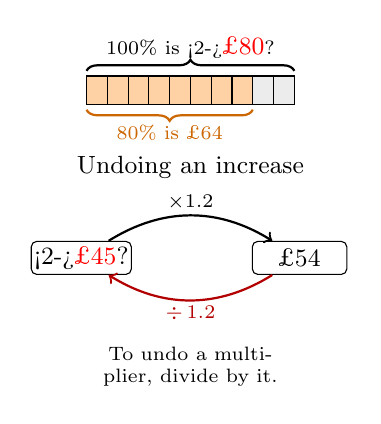
\begin{tikzpicture}[scale=0.66, every node/.style={font=\scriptsize}]

% ---- Reverse decrease shown as a bar model ----
\draw[topbrace] (0,0.30) -- (4.0,0.30);
\node at (2.0,0.75) {$100\%$ is \ashowq{\pounds80}};
\foreach \i in {0,...,9}{
  \ifnum\i<8
    \fill[orange!35] (\i*0.4,-0.35) rectangle ++(0.4,0.55);
  \else
    \fill[gray!15] (\i*0.4,-0.35) rectangle ++(0.4,0.55);
  \fi
  \draw (\i*0.4,-0.35) rectangle ++(0.4,0.55);
}
\draw[bottombrace, orange!80!black] (3.2,-0.45) -- (0,-0.45);
\node[orange!80!black] at (1.6,-0.90) {$80\%$ is \pounds64};

% ---- Reverse increase shown as a flow chart ----
\node[font=\small] at (2.0,-1.55) {Undoing an increase};
\node[rbox] (t0) at (-0.1,-3.30) {\ashowq{\pounds45}};
\node[rbox] (t1) at ( 4.1,-3.30) {\pounds54};
\draw[fwdarc] (t0) to node[flab, above] {$\times 1.2$} (t1);
\draw[bckarc] (t1) to node[flab, below] {$\div\, 1.2$} (t0);
\node[font=\scriptsize, text width=3.9cm, align=center] at (2.0,-5.40)
  {To undo a multiplier, divide by it.};

\end{tikzpicture}
\end{center}

\column{0.64\textwidth}
\vspace{-1.8em}
\footnotesize
\begin{enumerate}\tightlist
\begin{multicols}{2}
  \item Write $\dfrac{5}{8}$ as a decimal and as a percentage.
        \ashow{$0.625 = 62.5\%$}
  \columnbreak
  \item Write $24\%$ as a fraction in its simplest form.
        \ashow{$\tfrac{24}{100}=\tfrac{6}{25}$}
\end{multicols}
  \item A price is reduced by $20\%$ to \pounds64. Complete the chain from the bar model.
  \vspace{-0.2em}
  \begin{center}
    $80\%$ is \pounds64\\[1pt]
    $10\%$ is \ablank{\pounds8}\\[1pt]
    $100\%$ is \ablank{\pounds80}
  \end{center}
  \vspace{-0.2em}
  \item A price is increased by $20\%$ to \pounds54. Write the original price in the empty box of
        the flow chart.
        \ashow{$54\div1.2=$ \pounds45}
\begin{multicols}{2}
  \item A jacket costs \pounds68 after a $15\%$ reduction. Find the original price.
        \ashow{$68\div0.85=$ \pounds80}
  \columnbreak
  \item A salary rises by $4\%$ to \pounds33\,280. Find the salary before the rise.
        \ashow{$33\,280\div1.04=$ \pounds32\,000}
\end{multicols}
  \item Sam says ``a coat reduced by $25\%$ costs \pounds60, so the original price was
        $60+25\%$ of $60=$ \pounds75''. Explain Sam's mistake and find the correct original price.
        \ashow{The $25\%$ was taken off the original price, not off \pounds60. \pounds60 is $75\%$, so $60\div0.75=$ \pounds80.}
\end{enumerate}
\end{columns}
\end{frame}

%------------------------------------------------------------------
% STARTER 4: Simple and compound interest
%------------------------------------------------------------------
\begin{frame}[t]{Retrieve and Connect}
\begin{columns}[T]

\column{0.40\textwidth}
\begin{center}
\vspace{-0.4em}
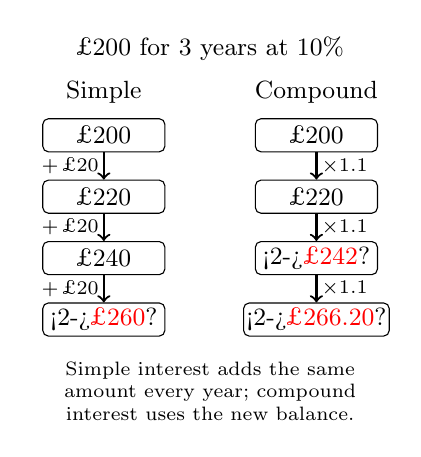
\begin{tikzpicture}[scale=1, every node/.style={font=\scriptsize}]

\node[font=\small] at (1.35,0.75) {\pounds200 for 3 years at $10\%$};

% ---- Simple interest ----
\node[font=\small] at (0,0.20) {Simple};
\node[fbox] (s0) at (0,-0.35) {\pounds200};
\node[fbox] (s1) at (0,-1.13) {\pounds220};
\node[fbox] (s2) at (0,-1.91) {\pounds240};
\node[fbox] (s3) at (0,-2.69) {\ashowq{\pounds260}};
\draw[farrow] (s0) -- node[flab,left] {$+\,$\pounds20} (s1);
\draw[farrow] (s1) -- node[flab,left] {$+\,$\pounds20} (s2);
\draw[farrow] (s2) -- node[flab,left] {$+\,$\pounds20} (s3);

% ---- Compound interest ----
\node[font=\small] at (2.7,0.20) {Compound};
\node[fbox] (c0) at (2.7,-0.35) {\pounds200};
\node[fbox] (c1) at (2.7,-1.13) {\pounds220};
\node[fbox] (c2) at (2.7,-1.91) {\ashowq{\pounds242}};
\node[fbox] (c3) at (2.7,-2.69) {\ashowq{\pounds266.20}};
\draw[farrow] (c0) -- node[flab,right] {$\times 1.1$} (c1);
\draw[farrow] (c1) -- node[flab,right] {$\times 1.1$} (c2);
\draw[farrow] (c2) -- node[flab,right] {$\times 1.1$} (c3);

\node[font=\scriptsize, text width=4.4cm, align=center] at (1.35,-3.60)
  {Simple interest adds the same amount every year;
   compound interest uses the new balance.};

\end{tikzpicture}

\vspace{0.4em}
{\scriptsize
\begin{tabular}{c|c|c}
  Year & Simple & Compound\\ \hline
  1 & \pounds220 & \pounds220\\
  2 & \pounds240 & \ablank{\pounds242}\\
  3 & \ablank{\pounds260} & \ablank{\pounds266.20}
\end{tabular}}
\end{center}

\column{0.60\textwidth}
\vspace{-1.8em}
\footnotesize
\begin{enumerate}\tightlist
\begin{multicols}{2}
  \item Write $3\%$ as a decimal and $0.045$ as a percentage.
        \ashow{$0.03$ and $4.5\%$}
  \columnbreak
  \item Write $\dfrac{1}{40}$ as a percentage.
        \ashow{$2.5\%$}
\end{multicols}
  \item Write the missing balances in the boxes and in the table.
\begin{multicols}{2}
  \item Find the simple interest on \pounds1200 at $5\%$ for 4 years.
        \ashow{\pounds60 a year, so \pounds240}
  \columnbreak
  \item Find the value of \pounds4000 after 5 years at $3\%$ compound interest.
        \ashow{$4000\times1.03^{5}=$ \pounds4637.10}
\end{multicols}
  \item Ravi saves \pounds300 for 3 years at either $6\%$ simple or $5\%$ compound.
        Which pays more?
        \ashow{A: \pounds354; B: $300\times1.05^{3}=$ \pounds347.29, so A pays more.}
  \item Account A pays $10\%$ simple but holds at most \pounds300. Account B pays $5\%$ simple,
        no maximum. Dev saves \pounds1000 for 3 years. Which is better, and by how much?
        \ashow{A: \pounds390 plus the \pounds700 that earns nothing, so \pounds1090.
               B: \pounds1150, so B by \pounds60.}
\end{enumerate}
\end{columns}
\end{frame}

%------------------------------------------------------------------
% STARTER 5: Reading interest from a graph
%------------------------------------------------------------------
\begin{frame}[t]{Retrieve and Connect}
\begin{columns}[T]

\column{0.38\textwidth}
\begin{center}
\vspace{-0.4em}
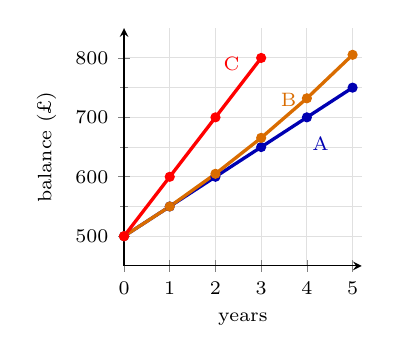
\begin{tikzpicture}
\begin{axis}[
  width=4.6cm, height=4.6cm,
  xlabel={years}, ylabel={balance (\pounds)},
  xlabel style={font=\scriptsize}, ylabel style={font=\scriptsize},
  tick label style={font=\scriptsize},
  xmin=0, xmax=5.2, ymin=450, ymax=850,
  xtick={0,1,2,3,4,5}, ytick={500,600,700,800},
  minor y tick num=1,
  grid=both, grid style={black!12},
  axis lines=left,
]
  \addplot[blue!70!black, very thick, mark=*, mark size=1.2pt]
    coordinates {(0,500)(1,550)(2,600)(3,650)(4,700)(5,750)};
  \addplot[orange!85!black, very thick, mark=*, mark size=1.2pt]
    coordinates {(0,500)(1,550)(2,605)(3,665.5)(4,732.05)(5,805.26)};
  \node[blue!70!black, font=\scriptsize] at (axis cs:4.3,655) {A};
  \node[orange!85!black, font=\scriptsize] at (axis cs:3.6,730) {B};
  \only<2->{%
    \addplot[red, very thick, mark=*, mark size=1.2pt]
      coordinates {(0,500)(1,600)(2,700)(3,800)};
    \node[red, font=\scriptsize] at (axis cs:2.35,790) {C};}
\end{axis}
\end{tikzpicture}\\[-0.4em]
{\scriptsize Both accounts start with \pounds500.}
\end{center}

\column{0.62\textwidth}
\vspace{-1.8em}
\footnotesize
\begin{enumerate}\tightlist
\begin{multicols}{2}
  \item Write $1.08$ as a percentage and $0.6\%$ as a decimal.
        \ashow{$108\%$ and $0.006$}
  \columnbreak
  \item Write $0.45$ as a fraction in its simplest form.
        \ashow{$\tfrac{45}{100}=\tfrac{9}{20}$}
\end{multicols}
\begin{multicols}{2}
  \item Both accounts pay the same rate. Use the graph to find it.
        \ashow{After 1 year both hold \pounds550, so \pounds50 on \pounds500, a rate of $10\%$}
  \columnbreak
  \item Which account pays simple interest, and how can you tell?
        \ashow{A, because it rises by the same \pounds50 every year, so the graph is a straight line}
\end{multicols}
  \item Account C pays $20\%$ simple interest on \pounds500. Complete the table, then plot the four
        points on the graph.
  \vspace{0.2em}
  \begin{center}
  \begin{tabular}{c|c|c|c|c}
    Years & 0 & 1 & 2 & 3\\ \hline
    Balance & \pounds500 & \ablank{\pounds600} & \ablank{\pounds700} & \ablank{\pounds800}
  \end{tabular}
  \end{center}
  \vspace{0.3em}
  \item An account pays $2\%$ compound interest every 6 months. Is that the same as $4\%$ a year?
        Explain your answer.
        \ashow{No. $1.02\times1.02=1.0404$, so the year's multiplier is $1.0404$ and the rate is $4.04\%$.}
\end{enumerate}
\end{columns}
\end{frame}

\end{document}
